\documentclass[11pt,a4paper]{article}
\usepackage[margin=2.5cm,headheight=15pt]{geometry}
\usepackage{amsmath,amssymb,amsthm}
\usepackage{mathtools}
\usepackage{microtype}
\usepackage{hyperref}
\usepackage{cleveref}
\usepackage{enumitem}
\usepackage{mdframed}
\usepackage{xcolor}
\usepackage{titlesec}
\usepackage{booktabs}
\usepackage{listings}
\usepackage{tikz}
\usetikzlibrary{positioning,arrows.meta,shapes.geometric,calc}
\usepackage{fancyhdr}

\definecolor{navyblue}{RGB}{26,58,92}
\definecolor{midblue}{RGB}{44,95,138}
\definecolor{lightblue}{RGB}{232,240,248}
\definecolor{proofgray}{RGB}{242,242,242}

\hypersetup{colorlinks=true,linkcolor=midblue,citecolor=midblue,urlcolor=midblue}

\pagestyle{fancy}\fancyhf{}
\fancyhead[L]{\small\color{navyblue}\textit{SSP Foundations: Formulations, KTNS, LP Analysis}}
\fancyhead[R]{\small\color{navyblue}\thepage}
\renewcommand{\headrulewidth}{0.4pt}

\titleformat{\section}{\large\bfseries\color{navyblue}}{}{0em}{}[\color{navyblue}\titlerule]
\titleformat{\subsection}{\normalsize\bfseries\color{midblue}}{}{0em}{}
\titleformat{\subsubsection}{\normalsize\itshape\color{midblue}}{}{0em}{}

\newmdenv[backgroundcolor=lightblue,linecolor=navyblue,linewidth=1.2pt,
  leftline=true,rightline=false,topline=false,bottomline=false,
  innerleftmargin=12pt,innerrightmargin=8pt,innertopmargin=8pt,
  innerbottommargin=8pt,skipabove=10pt,skipbelow=6pt]{thmbox}

\newmdenv[backgroundcolor=proofgray,linecolor=midblue,linewidth=0.8pt,
  leftline=true,rightline=false,topline=false,bottomline=false,
  innerleftmargin=10pt,innerrightmargin=8pt,innertopmargin=6pt,
  innerbottommargin=6pt,skipabove=6pt,skipbelow=6pt]{proofbox}

\theoremstyle{plain}
\newtheorem{theorem}{Theorem}[section]
\newtheorem{lemma}[theorem]{Lemma}
\newtheorem{proposition}[theorem]{Proposition}
\newtheorem{corollary}[theorem]{Corollary}
\theoremstyle{definition}
\newtheorem{definition}[theorem]{Definition}
\newtheorem{remark}[theorem]{Remark}

\setlist[itemize]{noitemsep,topsep=4pt}
\setlist[enumerate]{noitemsep,topsep=4pt}

% ─────────────────────────────────────────────────────────────────────────────
\begin{document}
% ─────────────────────────────────────────────────────────────────────────────

\begin{center}
  {\color{navyblue}\rule{\textwidth}{2pt}}\\[0.4cm]
  {\LARGE\bfseries\color{navyblue}The Job Sequencing and Tool Switching Problem}\\[0.3cm]
  {\large\itshape\color{midblue}Part I: Foundations — Formulations, KTNS, and LP Analysis}\\[0.2cm]
  {\color{navyblue}\rule{\textwidth}{2pt}}
\end{center}

\begin{mdframed}[backgroundcolor=lightblue,linecolor=navyblue,linewidth=1pt,
  innerleftmargin=14pt,innerrightmargin=14pt,innertopmargin=8pt,innerbottommargin=8pt]
\small\textbf{Scope.}
This document covers the established theoretical foundations of the Uniform
Job Sequencing and Tool Switching Problem (U-SSP): the formal problem definition,
the Tang--Denardo decomposition, the KTNS optimal tooling policy, and a rigorous
analysis of why classical compact ILP formulations fail computationally.
All results in this document are from the literature and are attributed accordingly.
\end{mdframed}

\vspace{0.5cm}
\tableofcontents
\newpage

% ─────────────────────────────────────────────────────────────────────────────
\section{Problem Definition: The Uniform SSP}
\label{sec:definition}
% ─────────────────────────────────────────────────────────────────────────────

A Flexible Manufacturing System (FMS) consists of a CNC machine with an
automated tool changer and a magazine of limited capacity $b$.
The machine must process a set of $n$ jobs sequentially, where each job requires
a specific subset of tools to be simultaneously loaded in the magazine.
Since the total number of distinct tools $m$ typically exceeds $b$, tools must
be swapped in and out as the machine moves from job to job. Each individual tool
swap incurs a time penalty. The \emph{Uniform SSP} asks: in what order should
the jobs be processed, and which tools should be in the magazine at each step,
so that the total number of tool switches is minimised?

\subsection{Formal Setup}

Let $J = \{1,2,\ldots,n\}$ be the set of jobs and $T = \{1,2,\ldots,m\}$ the set
of all available tools. The machine has magazine capacity $b \in \mathbb{Z}^+$
with $b < m$. Each job $j \in J$ requires the tool subset $T_j \subseteq T$, and
we assume $|T_j| \le b$ for all $j$ (otherwise the instance is infeasible).

The \emph{job-tool incidence matrix} $\mathbf{A} \in \{0,1\}^{m \times n}$ encodes
these requirements:
\[
  a_{tj} = \begin{cases} 1 & \text{if } t \in T_j, \\ 0 & \text{otherwise.} \end{cases}
\]

\begin{definition}[Feasible magazine sequence]
A sequence of magazine states $\mathcal{M} = (M_1, M_2, \ldots, M_n)$ is
\emph{feasible} for job permutation $\sigma \in \Sigma_n$ if, for every step $k$:
\[
  |M_k| \le b \quad \text{and} \quad T_{\sigma(k)} \subseteq M_k.
\]
\end{definition}

The cost of transitioning from state $M_{k-1}$ to $M_k$ is the number of
tool insertions required:
\[
  \mathrm{cost}(M_{k-1} \to M_k) = |M_k \setminus M_{k-1}|.
\]

\begin{definition}[U-SSP objective]
Find a permutation $\sigma^* \in \Sigma_n$ and a feasible magazine sequence
$\mathcal{M}^*$ minimising
\[
  Z_{\mathrm{SSP}}^* \;=\; \min_{\sigma,\,\mathcal{M}} \sum_{k=1}^{n-1} |M_{k+1} \setminus M_k|.
\]
\end{definition}

\begin{remark}
The U-SSP is \textbf{strongly NP-hard} \cite{Crama1994}: it subsumes the Hamiltonian
cycle problem. Even the tooling subproblem (optimal tool loading for a \emph{fixed}
sequence) is polynomial \cite{Tang1988}, as shown below.
\end{remark}

% ─────────────────────────────────────────────────────────────────────────────
\section{Maximal Configurations and Dummy Tool Padding}
\label{sec:maximal}
% ─────────────────────────────────────────────────────────────────────────────

In practice a job may require fewer tools than $b$, leaving slack slots. A key
structural lemma says we can always saturate those slots with \emph{dummy} tools
without increasing cost.

\begin{thmbox}
\begin{lemma}[Optimality of maximal configurations \cite{Tang1988}]
\label{lem:maximal}
For any feasible magazine sequence $\mathcal{M}$, there exists a sequence of
\emph{maximal} configurations $\mathcal{C} = (C_1,\ldots,C_n)$ with $|C_k|=b$
and $T_{\sigma(k)} \subseteq C_k$ for all $k$, whose total switching cost is
$\le$ that of $\mathcal{M}$.
\end{lemma}
\end{thmbox}

\begin{proofbox}
\begin{proof}
It suffices to show that padding a single under-capacity state $M_k$ with
$|M_k| < b$ by one tool never increases cost.
We identify the best tool to add by considering two cases.

\medskip\noindent\textit{Case 1: retain a tool from the previous state.}
Pick any $t \in M_{k-1} \setminus M_k$ and set $M'_k = M_k \cup \{t\}$.
The inflow cost $|M'_k \setminus M_{k-1}| = |M_k \setminus M_{k-1}|$ is unchanged
(because $t$ was already in $M_{k-1}$).
The outflow cost $|M_{k+1} \setminus M'_k| \le |M_{k+1} \setminus M_k|$
(since $M'_k \supset M_k$).
Net change $\le 0$.

\medskip\noindent\textit{Case 2: pre-load a future tool.}
If $M_{k-1} \subseteq M_k$, pick $t \in M_{k+1} \setminus M_k$ and set
$M'_k = M_k \cup \{t\}$.
Inflow cost increases by $+1$ (since $t \notin M_{k-1}$).
Outflow cost decreases by $-1$ (since $t \in M_{k+1}$). Net change $= 0$.

\medskip\noindent\textit{Case 3: arbitrary padding.}
If both adjacent sets are already subsets of $M_k$, any dummy tool can be added;
the net change is also $0$.

Applying this padding iteratively to every under-capacity state yields a maximal
sequence with cost $\le$ the original. \qed
\end{proof}
\end{proofbox}

\noindent\textbf{Consequence.} The search space can be restricted to
maximal configurations of size exactly $b$ without loss of generality.

% ─────────────────────────────────────────────────────────────────────────────
\section{The Tang--Denardo Decomposition}
\label{sec:decomposition}
% ─────────────────────────────────────────────────────────────────────────────

A central insight of \cite{Tang1988} is that the U-SSP decomposes into two
nested subproblems.

\begin{definition}[Sequencing Problem (SP)]
Given job set $J$, find the permutation $\sigma^* \in \Sigma_n$ that minimises
the cost of the inner Tooling Problem.
\end{definition}

\begin{definition}[Tooling Problem (TP)]
Given a fixed permutation $\sigma$, find the sequence of maximal magazine
configurations $(C_1,\ldots,C_n)$ with $T_{\sigma(k)} \subseteq C_k$ and $|C_k|=b$
that minimises
\[
  TP(\sigma) \;=\; \min_{\mathcal{C}} \sum_{k=1}^{n-1} |C_{k+1} \setminus C_k|.
\]
\end{definition}

The global objective is therefore $Z_{\mathrm{SSP}}^* = \min_{\sigma} TP(\sigma)$.
The decomposition reveals two critical structural facts:

\begin{enumerate}
\item The TP is \textbf{solvable in polynomial time} for any fixed $\sigma$
      (via the KTNS algorithm described next).
\item The SP \textbf{cannot} be solved by static TSP-style edge weights, because
      the transition cost from job $i$ to job $j$ depends on the full history of
      the magazine state leading up to that transition.
\end{enumerate}

\begin{proposition}[Failure of static greedy sequencing \cite{Tang1988}]
\label{prop:greedy_fail}
Any algorithm that sequences jobs using fixed, precomputed edge costs
$c_{ij} = \max\{0, |T_i \cup T_j| - b\}$ cannot guarantee global optimality for
the U-SSP.
\end{proposition}

\begin{proofbox}
\begin{proof}
The cost $c_{ij}$ is the \emph{minimum} number of switches required to process
job $j$ immediately after job $i$ in a two-job subsequence, ignoring the magazine
contents inherited from earlier jobs. In reality, the optimal tooling policy for a
long prefix fills the slack slots $C_k \setminus T_{\sigma(k)}$ with tools needed
by future jobs. A greedy algorithm evaluating only $c_{ij}$ is blind to these
pre-loaded tools. It may select a successor job $j'$ that appears cheaper under
$c_{ij'}$ but causes subsequent transitions to be far more expensive because the
look-ahead pre-load is destroyed. The true cost is thus a function of the entire
prefix permutation, not a pairwise quantity. \qed
\end{proof}
\end{proofbox}

% ─────────────────────────────────────────────────────────────────────────────
\section{Interval Matrices and the KTNS Policy}
\label{sec:ktns}
% ─────────────────────────────────────────────────────────────────────────────

\subsection{0-Blocks and the Interval Property}

Fix a permutation $\sigma$ and consider the permuted incidence matrix
$\mathbf{A}^\sigma \in \{0,1\}^{m \times n}$ whose columns are ordered by $\sigma$.

\begin{definition}[0-block]
A \emph{0-block} for tool $t$ is a maximal contiguous run of zeros in row $t$ of
$\mathbf{A}^\sigma$ that is bounded on both sides by a 1. The interval $[k_1,k_2]$
is a 0-block if $a^\sigma_{t,k}=0$ for $k\in[k_1,k_2]$, while $a^\sigma_{t,k_1-1}=1$
and $a^\sigma_{t,k_2+1}=1$.
\end{definition}

A 0-block represents an idle window during which tool $t$ is not required, yet will
be needed again later. The decision to \emph{retain} $t$ across this gap (``flipping''
the 0-block) avoids a future re-insertion but occupies a magazine slot in the meantime.
If every 0-block of every tool is flipped, the matrix has the \emph{Consecutive Ones
Property (COP)}: all 1s in each row form a single contiguous block. Such matrices are
called \emph{interval matrices} and are \textbf{totally unimodular}, so the TP LP
relaxation has integer optimal solutions \cite{Crama1994}.

\subsection{The Keep Tool Needed Soonest (KTNS) Algorithm}

The KTNS policy resolves the TP optimally: whenever a slot must be freed to load a
required tool, evict the resident tool whose \emph{next} required use is
\emph{furthest in the future}. Let
\[
  L(t,k) = \min\{s \ge k : t \in T_{\sigma(s)}\}
\]
denote the next requirement step for tool $t$ at or after step $k$
(set to $n+1$ if $t$ is never needed again).

\begin{mdframed}[backgroundcolor=lightblue,linecolor=navyblue,linewidth=1.2pt,
  innerleftmargin=14pt,innerrightmargin=14pt,innertopmargin=10pt,innerbottommargin=10pt]
\textbf{Algorithm~1: Keep Tool Needed Soonest (KTNS)}

\smallskip
\textbf{Input:} Permutation $\sigma \in \Sigma_n$, requirement sets $T_{\sigma(k)}$, capacity $b$.\\
\textbf{Output:} Optimal magazine sequence $(C_1,\ldots,C_n)$ and cost $Z_{TP}$.

\medskip
\begin{enumerate}[noitemsep,label=\textbf{\arabic*.}]
\item Precompute $L(t,k) = \min\{s \ge k : t \in T_{\sigma(s)}\}$ for all $t \in T$,
      $k \in \{1,\ldots,n\}$. Set $L(t,k)=n+1$ if $t$ is never needed from $k$ onward.
\item Set $C_1 \leftarrow T_{\sigma(1)}$; pad to size $b$ by adding tools with the
      smallest values of $L(\cdot,1)$. Set $Z_{TP} \leftarrow 0$.
\item \textbf{For} $k = 2, 3, \ldots, n$:
  \begin{enumerate}[noitemsep,label=\alph*.]
    \item Set $C_k \leftarrow C_{k-1}$ (inherit the previous magazine state).
    \item \textbf{For each} required tool $t \in T_{\sigma(k)} \setminus C_k$:
      \begin{enumerate}[noitemsep,label=\roman*.]
        \item Choose the \textbf{KTNS eviction candidate}:
              $p \leftarrow \displaystyle\arg\max_{s \;\in\; C_k \setminus T_{\sigma(k)}} L(s,k)$
              \quad (evict the tool needed furthest in the future).
        \item Update: $C_k \leftarrow (C_k \setminus \{p\}) \cup \{t\}$.
              Increment: $Z_{TP} \leftarrow Z_{TP} + 1$.
      \end{enumerate}
  \end{enumerate}
\item \textbf{Return} $(C_1, C_2, \ldots, C_n)$ and $Z_{TP}$.
\end{enumerate}
\end{mdframed}
\vspace{4pt}
\noindent\textbf{Time complexity:} $O(n \cdot m \cdot b)$.\label{alg:ktns}

\begin{remark}
KTNS runs in $O(n \cdot m \cdot b)$ time and is analogous to Belady's
optimal page-replacement algorithm \cite{Belady1966}.
\end{remark}

\subsection{Optimality of KTNS}

\begin{thmbox}
\begin{theorem}[KTNS is optimal for the TP \cite{Tang1988}]
\label{thm:ktns}
For any fixed permutation $\sigma$ and capacity $b$, KTNS produces a magazine
sequence achieving the minimum switching cost $TP(\sigma)$.
\end{theorem}
\end{thmbox}

\begin{proofbox}
\begin{proof}
We use an exchange argument.
Let $\pi$ be any feasible tooling policy for $\sigma$.
We show how to transform $\pi$ step-by-step into KTNS without ever increasing cost.

\medskip
\noindent\textit{Setup.}
Let $k$ be the first step at which $\pi$ disagrees with KTNS.
At step $k$, a required tool $r \in T_{\sigma(k)} \setminus W_k$ must be inserted
(where $W_k$ is the shared magazine state just before the eviction), so one tool
from $W_k \setminus T_{\sigma(k)}$ must be evicted.
KTNS evicts $t^* = \arg\max_{s \in W_k \setminus T_{\sigma(k)}} L(s,k)$,
but $\pi$ evicts a different tool $s$ with $L(s,k) < L(t^*,k)$.

\medskip
\noindent\textit{Construction of $\pi'$.}
Define $\pi'$ identical to $\pi$ except that at step $k$ it evicts $t^*$ (agreeing
with KTNS). Let $p = L(s,k)$ and $q = L(t^*,k)$, so $p \le q$.

\medskip
\noindent\textit{Cost comparison during $[k,\,q]$.}
\begin{itemize}
\item \textbf{Step $k$}: both $\pi$ and $\pi'$ insert $r$ (one insertion each);
  the only difference is who else occupies the freed slot.
\item \textbf{Steps $k{+}1$ to $p{-}1$}: neither $s$ nor $t^*$ is required
  (since $p$ and $q$ are their next uses). Both policies are feasible and handle
  all other required tools identically; cost is the same.
\item \textbf{Step $p$} ($s$ first needed again):
  $\pi$ already has $s$ — no extra insertion.
  $\pi'$ does not have $s$ — must insert $s$ (+1 insertion for $\pi'$);
  $\pi'$ can evict $t^*$ (still unneeded until step $q$) to free the slot.
\item \textbf{Steps $p{+}1$ to $q{-}1$}: $t^*$ not needed yet. $\pi$ retains $t^*$;
  $\pi'$ does not have $t^*$. Both handle all other tools identically.
\item \textbf{Step $q$} ($t^*$ first needed again):
  If $\pi$ still has $t^*$: $\pi$ pays 0 for $t^*$; $\pi'$ must insert $t^*$
  (+1 insertion for $\pi'$).
  Net over $[k,q]$: $\pi'$ paid $+1$ at step $p$ and $+1$ at step $q$, while $\pi$
  paid $+1$ at step $p$ (for inserting $s$) and $0$ at step $q$.
  Total: $\pi'$ = 2 extra, $\pi$ = 1 extra — \textit{but we overcounted}.
\end{itemize}

\medskip
\noindent\textit{Correcting the count.}
The insertion of $r$ at step $k$ is paid by \emph{both} policies equally and does
not enter the comparison. The comparison reduces to:
\begin{center}
\begin{tabular}{lcc}
  \toprule
  Event & Policy $\pi$ & Policy $\pi'$ \\
  \midrule
  Insert $s$ at step $p$ & $+1$ & $0$ \\
  Insert $t^*$ at step $q$ & $0$ & $+1$ \\
  \bottomrule
\end{tabular}
\end{center}
The totals are equal: both policies pay exactly \textbf{1 insertion} for
the pair $\{s, t^*\}$ over the interval $[k,q]$.

If instead $\pi$ evicts $t^*$ before step $q$ (say at step $p$ when inserting $s$),
then $\pi$ also pays 1 for $t^*$ at step $q$ — again equal to $\pi'$.
In all cases, $\mathrm{cost}(\pi') \le \mathrm{cost}(\pi)$.

\medskip
\noindent\textit{Cascading differences.}
At step $p$, $\pi'$ evicts $t^*$ while $\pi$ may evict a different tool $u$.
This creates a new disagreement (in $u$) between $\pi$ and $\pi'$.
The same exchange argument applies to this new disagreement: evicting the
further-needed tool never increases cost.
Since the sequence has finite length $n$, applying the exchange argument
inductively reduces the number of disagreements to zero, transforming $\pi$ into
KTNS without increasing the total cost.
Hence $\mathrm{cost}(\text{KTNS}) \le \mathrm{cost}(\pi)$ for any feasible $\pi$,
proving KTNS is optimal. \qed
\end{proof}
\end{proofbox}

\subsection{Illustrated Example}

\begin{figure}[h!]
\centering
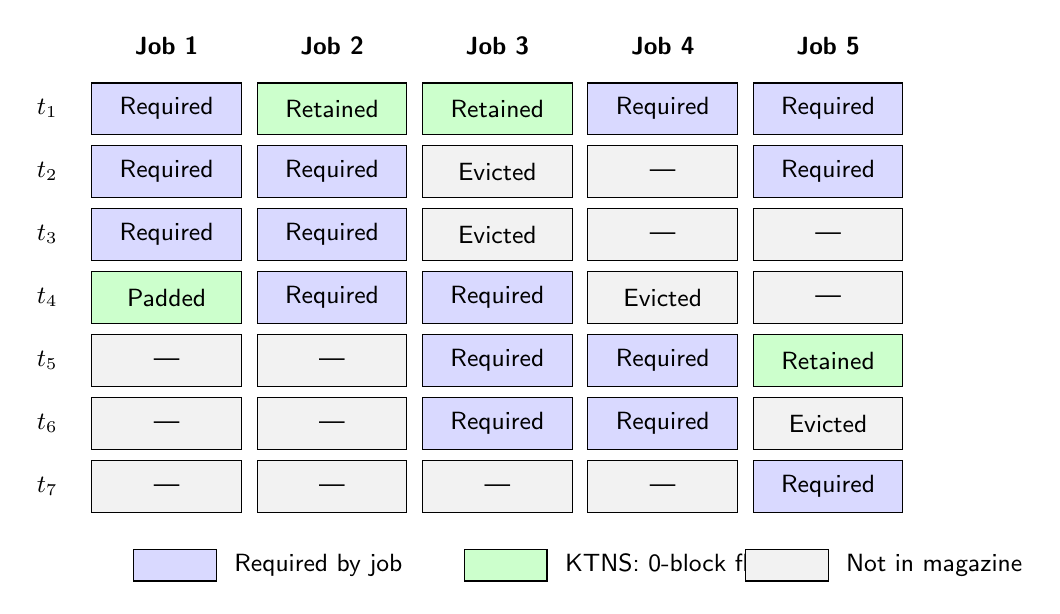
\begin{tikzpicture}[x=2.1cm, y=0.8cm, >=Stealth]
  \tikzset{
    req/.style={draw=black,fill=blue!15,minimum width=1.9cm,
                minimum height=0.65cm,font=\sffamily\small},
    ret/.style={draw=black,fill=green!20,minimum width=1.9cm,
                minimum height=0.65cm,font=\sffamily\small},
    emp/.style={draw=black,fill=gray!10,minimum width=1.9cm,
                minimum height=0.65cm,font=\sffamily\small},
    lbl/.style={font=\sffamily\bfseries\small}
  }
  % Column headers
  \foreach \j/\x in {1/1,2/2,3/3,4/4,5/5}
    \node[lbl] at (\x,0) {Job \j};
  % Row headers
  \foreach \t/\y in {$t_1$/-1,$t_2$/-2,$t_3$/-3,$t_4$/-4,$t_5$/-5,
                      $t_6$/-6,$t_7$/-7}
    \node[lbl,anchor=east] at (0.4,\y) {\t};
  % t1: required at 1,4,5; retained 2,3
  \node[req] at (1,-1) {Required}; \node[ret] at (2,-1) {Retained};
  \node[ret] at (3,-1) {Retained}; \node[req] at (4,-1) {Required};
  \node[req] at (5,-1) {Required};
  % t2: required at 1,2,5; evicted at 3 (capacity full)
  \node[req] at (1,-2) {Required}; \node[req] at (2,-2) {Required};
  \node[emp] at (3,-2) {Evicted};  \node[emp] at (4,-2) {---};
  \node[req] at (5,-2) {Required};
  % t3: required at 1,2; no future use
  \node[req] at (1,-3) {Required}; \node[req] at (2,-3) {Required};
  \node[emp] at (3,-3) {Evicted};  \node[emp] at (4,-3) {---};
  \node[emp] at (5,-3) {---};
  % t4: required at 2,3
  \node[ret] at (1,-4) {Padded};   \node[req] at (2,-4) {Required};
  \node[req] at (3,-4) {Required}; \node[emp] at (4,-4) {Evicted};
  \node[emp] at (5,-4) {---};
  % t5: required at 3,4; retained at 5
  \node[emp] at (1,-5) {---};      \node[emp] at (2,-5) {---};
  \node[req] at (3,-5) {Required}; \node[req] at (4,-5) {Required};
  \node[ret] at (5,-5) {Retained};
  % t6: required at 3,4
  \node[emp] at (1,-6) {---};      \node[emp] at (2,-6) {---};
  \node[req] at (3,-6) {Required}; \node[req] at (4,-6) {Required};
  \node[emp] at (5,-6) {Evicted};
  % t7: required at 5 only
  \node[emp] at (1,-7) {---};      \node[emp] at (2,-7) {---};
  \node[emp] at (3,-7) {---};      \node[emp] at (4,-7) {---};
  \node[req] at (5,-7) {Required};
  % Legend
  \draw[fill=blue!15] (0.8,-8.5) rectangle (1.3,-8.0);
  \node[anchor=west,font=\sffamily\small] at (1.35,-8.25) {Required by job};
  \draw[fill=green!20] (2.8,-8.5) rectangle (3.3,-8.0);
  \node[anchor=west,font=\sffamily\small] at (3.35,-8.25) {KTNS: 0-block flipped};
  \draw[fill=gray!10] (4.5,-8.5) rectangle (5.0,-8.0);
  \node[anchor=west,font=\sffamily\small] at (5.05,-8.25) {Not in magazine};
\end{tikzpicture}
\caption{KTNS magazine evolution for a 5-job, 7-tool instance ($b=4$).
Tool $t_1$ is retained across jobs 2--3 (0-block flipped) because capacity allows it.
Tool $t_2$'s 0-block cannot be flipped at job 3 because $T_3=\{t_4,t_5,t_6\}$ plus
the retained $t_1$ already saturates all 4 slots; $t_2$ must be evicted and
re-inserted before job 5.}
\label{fig:ktns}
\end{figure}

% ─────────────────────────────────────────────────────────────────────────────
\section{Compact ILP Formulations}
\label{sec:compact}
% ─────────────────────────────────────────────────────────────────────────────

Early exact approaches modelled the SSP as a single Integer Linear Program over
positional or arc-flow variables. We survey the four main formulations.

\subsection{Tang--Denardo Position-Based Model \cite{Tang1988}}

\noindent\textbf{Variables.}
\begin{itemize}
\item $u_{jk} \in \{0,1\}$: 1 if job $j$ is assigned to position $k$.
\item $v_{kt} \in \{0,1\}$: 1 if tool $t$ is in the magazine at position $k$.
\item $w_{kt} \ge 0$: number of insertions of tool $t$ at position $k$.
\end{itemize}
\begin{align}
\min \quad & \sum_{k,t} w_{kt} \label{eq:td_obj}\\
\text{s.t.}\quad
& \sum_k u_{jk} = 1 \;\;\forall j,\quad
  \sum_j u_{jk} = 1 \;\;\forall k \label{eq:td_perm}\\
& v_{kt} \ge \sum_j a_{tj}\,u_{jk} \;\;\forall k,t \label{eq:td_cov}\\
& \sum_t v_{kt} \le b \;\;\forall k \label{eq:td_cap}\\
& w_{kt} \ge v_{kt} - v_{k-1,t} \;\;\forall k,t \label{eq:td_sw}\\
& u_{jk},v_{kt} \in \{0,1\},\; w_{kt} \ge 0 \notag
\end{align}
Boundary condition: $v_{0,t} = 0$ for all $t$.
%% TODO-VERIFY(Claude-Fable 2026-06-10): convention remark added — with v_0 = 0
%% this ILP charges the initial load (EMPTY-START), while the U-SSP objective of
%% Section 1 is FREE-INITIAL. The two differ by the constant min(b,|U|) for every
%% sequence (argmin-safe); cf. the convention audit in Part VIII.
\emph{Convention note: with $v_{0,t}=0$ this model charges the initial loading
(empty-start); its optimum exceeds the free-initial $Z^{*}_{\mathrm{SSP}}$ of
\S\,1 by exactly $\min(b,|U|)$, a sequence-independent constant.}

\subsection{Laporte--Salazar--Semet Arc-Flow Model \cite{Laporte2004}}

This model embeds the SP in an ATSP framework over jobs $J_0 = J \cup \{0\}$
(with dummy depot 0). Variables: $x_{ij} \in \{0,1\}$ (routing arc),
$y_{tj} \in \{0,1\}$ (tool $t$ present at job $j$),
$z_{tj} \in \{0,1\}$ (tool $t$ inserted at job $j$).
\begin{align}
\min \quad & \sum_{j,t} z_{tj} \notag\\
\text{s.t.}\quad
& \sum_{i \ne j} x_{ij} = \sum_{i \ne j} x_{ji} = 1 \;\;\forall j \label{eq:lap_deg}\\
& \text{Subtour elimination constraints (SECs)} \notag\\
& y_{tj} \ge a_{tj} \;\;\forall j,t \label{eq:lap_cov}\\
& \sum_t y_{tj} \le b \;\;\forall j \label{eq:lap_cap}\\
& z_{tj} \ge y_{tj} - y_{ti} + x_{ij} - 1
  \;\;\forall i \ne j,\, \forall t \label{eq:lap_sw}
\end{align}
Constraint~\eqref{eq:lap_sw} avoids Big-M: if $x_{ij}=1$ (job $j$ directly
follows $i$) it forces $z_{tj} \ge y_{tj} - y_{ti}$,
i.e., tool $t$ must be inserted at $j$ if it was absent at $i$.
When $x_{ij}=0$ the constraint is inactive.

\subsection{Catanzaro--Gouveia--Labbé Linear Ordering Model \cite{Catanzaro2015}}

Instead of absolute positions, binary variable $x_{ij}=1$ encodes that job $i$
is processed \emph{before} $j$ (not necessarily immediately). Tournament and
transitivity constraints enforce a valid linear order:
\begin{align}
& x_{ij} + x_{ji} = 1 \;\;\forall i \ne j \label{eq:cat_tourn}\\
& x_{ij} + x_{jk} + x_{ki} \le 2 \;\;\forall i \ne j \ne k \label{eq:cat_trans}
\end{align}
The objective maximises retained 0-blocks directly. A retention variable
$y^t_{ij}=1$ indicates that tool $t$ (required by both $i$ and $j$) is kept
continuously between $i$ and $j$ without any intermediate job needing it.
Overlap capacity constraints prevent the simultaneous retention of too many
tools at any intermediate job $k$:
\[
  \sum_{t \notin T_k}\sum_{i : t \in T_i}\sum_{j : t \in T_j}
  y^t_{ij}(x_{ik}+x_{kj}-1) \le b - |T_k|
  \quad \forall k \in J.
\]
%% TODO-VERIFY(Claude-Fable 2026-06-10): the displayed capacity condition is
%% QUADRATIC (y·x products) — a schematic only; the actual paper formulation is
%% linearised. Also "tightest among compact formulations" predates da Silva 2024.
(The display is schematic --- the paper's formulation linearises these products.)
This model achieved the tightest LP relaxation among the compact formulations of
its time \cite{Catanzaro2015}; the SSPMF below now provides the strongest known
root bound.

\subsection{Arc-Retention Flow Tightening; and the SSPMF}
%% TODO-VERIFY(Claude-Fable 2026-06-10): this subsection previously mislabelled an
%% arc-retention flow sketch (in the spirit of Catanzaro et al.'s y^t_{ij}
%% variables) as "SSPMF". The actual SSPMF (da Silva, Chaves & Yanasse 2024) is a
%% POSITION-based multicommodity flow model with proven root LP bound M-C — it
%% does NOT collapse to 0, contradicting the old text. Both are now described.

A first tightening treats tool continuity as a flow on the job-arc graph: for
each tool $t$, $f^t_{ij} \in \{0,1\}$ indicates that $t$ is continuously
retained across the direct arc $i \to j$, with
\[
  z_{tj} \ge y_{tj} - \sum_{i \ne j} f^t_{ij}
  \quad \forall j, t, \qquad \sum_t f^t_{ij} \le b \cdot x_{ij},
\]
in the spirit of the arc-based variables $y^t_{ij}$ of Catanzaro et
al.~\cite{Catanzaro2015} (Formulations 3/4), whose LP relaxation provably
dominates the Laporte model.

The \emph{SSPMF} proper (da Silva, Chaves \& Yanasse~\cite{daSilva2024}) is a
\emph{position-based} multicommodity flow model (one commodity per tool, flows
over a position-expanded graph). It is the notable \textbf{exception} to the LP
collapse of \cref{thm:lp_collapse}: its root LP bound is $M-C$ (tools minus
capacity), proven tight, and it currently solves the most benchmark instances.
It is implemented in \texttt{src/BBC/sspmf\_formulation.py}.

% ─────────────────────────────────────────────────────────────────────────────
\section{Why Compact Models Fail: LP Collapse and Symmetry}
\label{sec:lp_failure}
% ─────────────────────────────────────────────────────────────────────────────

All four compact models above suffer from two interrelated weaknesses that make
them computationally intractable beyond small instances.

\subsection{LP Lower Bound Collapse to Zero}

\begin{thmbox}
%% TODO-VERIFY(Claude-Fable 2026-06-10): citation corrected — the LP=0 proof for
%% the Tang–Denardo model is due to Laporte, Salazar-González & Semet (2004), §2.1
%% (see the literature skill), not Tang1988/Catanzaro2015.
\begin{theorem}[LP bound collapse \cite{Laporte2004}]
\label{thm:lp_collapse}
The LP relaxation of the Tang--Denardo position-based model admits a feasible
solution with objective value $0$, regardless of the true integer optimum.
\end{theorem}
\end{thmbox}

\begin{proofbox}
\begin{proof}
Set $u_{jk} = 1/n$ for all $j,k$; this satisfies the doubly-stochastic
assignment constraints~\eqref{eq:td_perm}. The coverage constraint~\eqref{eq:td_cov}
then forces
\[
  v_{kt} \ge \frac{1}{n}\sum_j a_{tj} \quad \forall k,t.
\]
Set $v_{kt} = \frac{1}{n}\sum_j a_{tj}$ (independent of $k$).
The capacity constraint~\eqref{eq:td_cap} is satisfied because
$\sum_t v_{kt} = \frac{1}{n}\sum_j |T_j| \le b$.
Since $v_{kt}$ is constant in $k$, the gradient $v_{kt}-v_{k-1,t}=0$ everywhere,
so the transition variables $w_{kt}=0$ are feasible.
The objective evaluates to $\sum_{k,t} w_{kt} = 0$. \qed
\end{proof}
\end{proofbox}

\begin{remark}
%% TODO-VERIFY(Claude-Fable 2026-06-10): scope of the collapse corrected — it
%% does NOT extend to the SSPMF (root LP = M−C, da Silva 2024), and Catanzaro's
%% F3/F4 also have provably positive LP bounds dominating Laporte's.
A similar smearing degrades the Laporte arc-flow LP (valid inequalities recover
some strength, e.g.\ bound $6.0$ vs.\ integer optimum $7$ on the Tang--Denardo
example~\cite{Laporte2004}). The collapse does \emph{not} extend to the stronger
models: Catanzaro's Formulations~3/4 and especially the SSPMF (root LP $=M-C$)
have provably positive bounds. The same uniform-blend pathology re-appears,
however, in any \emph{position-aggregated configuration} model --- see Part~X
(\texttt{10\_position\_formulations.tex}), where it is proved and repaired.
\end{remark}

\subsection{Exponential Symmetry from 0-Block Choices}

Even when variables are fixed to $\{0,1\}$, compact models suffer from
\emph{permutational symmetry}: the binary choice of whether to retain or evict
a tool during each 0-block generates exponentially many equivalent integer
solutions.

\begin{thmbox}
%% TODO-VERIFY(Claude-Fable 2026-06-10): the previous "theorem" here ("2^k equal-
%% cost 0-block choices") was FALSE: when capacity is slack, RETAINING a 0-block
%% strictly saves one re-insertion, so retain vs evict differ in cost by 1 — a
%% dominance, not a plateau. The genuine symmetry sources are stated below.
\begin{theorem}[Exponential integer symmetry of compact models]
\label{thm:symmetry}
Fix an optimal sequence and an optimal tooling plan in the Tang--Denardo model.
If at $k$ distinct positions the magazine has a free slot whose content is
irrelevant (at least two unused tools could occupy it without affecting any
future insertion), then at least $2^k$ integer assignments of the $(v,w)$
variables attain the optimal objective. Independently, the reversal of any
optimal sequence is optimal (Ghiani et al.'s symmetry property), doubling the
count again.
\end{theorem}
\end{thmbox}

\begin{proofbox}
\begin{proof}[Sketch]
Padding slots are free: a tool occupying a slack slot that is never required
before its eviction contributes no insertion beyond its (already counted)
loading, and exchanging which unused tool sits in the slot changes neither
feasibility nor cost; $k$ independent binary slot choices give $2^k$ equal-cost
assignments. Reversal symmetry preserves the total switch count (only the
per-transition split changes). Branch-and-bound must implicitly enumerate these
equivalent assignments unless symmetry-breaking constraints are added --- one
reason the SSPMF includes an explicit anchor (its Eq.~20).
\end{proof}
\end{proofbox}

\subsection{Combined Implication}

The LP collapse to 0 means the root-node bound gives no useful pruning
information. The $2^k$ symmetry means the search tree branches on
combinatorially equivalent choices at every node. Together, these render
all four compact formulations impractical for instances with more than
roughly 25 jobs \cite{Laporte2004,Catanzaro2015}. This motivates the
\emph{non-compact, configuration-based formulation} developed in the
companion document \texttt{02\_noncompact\_formulation.tex}.

%----------------------------------------------------------------------
\bibliographystyle{abbrvnat}
\bibliography{references}
%----------------------------------------------------------------------
\end{document}
